% Created 2015-11-24 Di 14:02
\documentclass{sig-alternate-05-2015}
\newif\iflong
\longfalse
\def\itemadjust{\vspace*{-2ex}}
                              %\pdfpagewidth=8.5truein
%\pdfpageheight=11truein
\usepackage[utf8]{inputenc}
\usepackage{amsmath}
\usepackage{hyperref}
\usepackage{natbib}
\usepackage{subfigure}
% \renewcommand{\textfraction}{0.05}
% \renewcommand{\topfraction}{0.99}
% \renewcommand{\floatpagefraction}{0.9}
\usepackage{color}
\usepackage{xspace}
\usepackage[table]{xcolor}
\definecolor{light-gray}{gray}{0.97}
\usepackage{listings}
\usepackage{listings-C}
\usepackage{listings-x86_64}
\usepackage{listings-modernC}
\lstloadlanguages{C11,C99}
\lstset{
language=[errnoPOSIX]{C},
language=[tgmath]{C},
language=[threads]{C},
language=[stdatomic]{C},
language=[boundschecking]{C},
language=[99]{C},
language={C11},
style=modernC,
basicstyle=\tt\scriptsize,
moreemph=[5]{
futex_wait,
futex_wake,
},
moreemph=[3]{
smpl_lock,
smpl_unlock,
smpl, ftx,
ftx_bit,
ftx_fetch_add,
ftx_cmpxch,
ftx_load,
ftx_lock,
ftx_unlock,
ftx_mask,
ftx_count,
ftx_set,
ftx_lkd,
ftx_contrib,
},
}
\newcommand{\code}[1]{\text{\lstinline`#1`\xspace}}
\author{Jens Gustedt\\
%  \affaddr{\framebox[1.5cm] and \framebox[3cm]{[\hfill]}, \framebox[5cm]{[\hfill]}, \framebox[3cm]{[\hfill]}}}
\affaddr{INRIA and ICube, Universit\'{e} de Strasbourg, France}}
%\setcopyright{acmcopyright}
\doi{http://dx.doi.org/xx.xxxx/xxxxxxx.xxxxxxx}
\isbn{978-1-4503-3739-7/16/04}
%\isbn{---}
%\conferenceinfo{PLDI '13}{June 16--19, 2013, Seattle, WA, USA}
%\acmPrice{\$15.00}
\conferenceinfo{SAC'16,}{ April 4-8, 2016, Pisa, Italy}
\CopyrightYear{2016} % Allows default copyright year (20XX) to be ove
% switch off the table of contents just for LaTeX export
\let\tableofcontents=\relax
% ensure that in the LaTeX output links are visible as footnotes
\let\oldHref=\href
\def\href#1#2{\oldHref{#1}{#2}\footnote{\url{#1}}}
\newtheorem{remark}{Remark}[section]
\newtheorem{lemma}[remark]{Lemma}
\newtheorem{theorem}[remark]{Theorem}
\date{\today}
\title{Futex based locks for C11's generic atomics%
  \thanks{A long version of this paper can be found in \cite{gustedt15:futex}}
\\
(extended abstract)}
\hypersetup{
    pdftitle={Futex based locks for C11's generic atomics, Extended Abstract},
    pdfauthor={Jens Gustedt},
    pdfkeywords={lock primitives, atomics, C11, futex, Linux},
    pdfsubject={Futex based locks for C11's generic atomics},
    bookmarksopen = true,
    pdflang={English},
}
\begin{document}

\maketitle
\tableofcontents


\begin{abstract}
We present a new algorithm and implementation of a lock primitive that
is based on Linux' native lock interface, the \texttt{futex} system
call. It allows us to assemble compiler support for atomic data
structures that can not be handled through specific hardware
instructions.  Such an implementation is needed for C11's atomics
interface because here an \code{_Atomic} qualification can be attached
to almost any data type. Our lock data structure for that purpose
meets very specific criteria concerning its field of operation and its
performance. By that we are able to outperform gcc's
\texttt{libatomic} library by around 60\%.

%%% Local Variables:
%%% mode: latex
%%% mode: reftex
%%% fill-column: 75
%%% ispell-dictionary: "american"
%%% x-symbol-8bits: nil
%%% End:

\end{abstract}



\section{Introduction}
\label{sec-1}

Only very recently (with C11, see \citeauthor{C11}) the C language has
integrated threads and atomic operations into the core of the
language.  Support for these features is still partial: where the
main open source compilers~\citeauthor{gcc} and~\citeauthor{clang} now offer atomics, most Linux
platforms still use~\citeauthor{glibc}
as their C library which does not implement C11 threads. Only
platforms that are based on~\citeauthor{musl} as C
library, e.g~\citeauthor{alpine}, are
feature complete.

The implementation of the C11 atomic interface typically sits in the
middle between the implementation of the core language
and the
C library. It needs compiler support for the individual atomic operations
and a \emph{generic atomic lock} interface in the C library when no
low-level atomic instruction is available.


Since Linux' open source C libraries do not implement the generic
interface, the compilers currently provide a library stub that
implements the necessary lock by means of a combination of atomics
and~\citeauthor{POSIX2009}
\code{pthread_mutex_t}.

From a point of view of the C language the natural interface
for that would be C11 threads,
but since these are still missing in \texttt{glibc}, they fall back to
POSIX threads,
%
instead of
%
mapping to platform specific properties
and drawing the best performance from a given platform. In
this work we present a specific algorithm for the generic lock that
relies on a specific Linux utility, the \texttt{futex} system
call.

A \texttt{futex} combines one atomic integer and OS scheduling.
In our approach, we
use one \code{unsigned} to
implement the lock and a waiter count at the same time.
The resulting data type of minimal size (32 bit on all
architectures) and the algorithm can take advantage
by minimizing the number of CPU to memory transfers. In most cases
one such transfer is sufficient, where other algorithms have to
update a lock and a waiter counter separately.

To our knowledge pursuing this approach to a complete solution is
new. Previously urban myth had it that such approaches would risk
deadlocks if confronted to heavy load, because repeated failures of
calls to \code{futex_wait} could lead to unbounded loops. We are able to
prove that such unbounded loops will not happen for our algorithm.
Also, our measurements have shown that such an approach can be very
effective: failed system calls to \code{futex_wait} are much less costly
than commonly thought.

Our algorithm and its implementation is part of a larger open source
project to provide the necessary interfaces (header files) and library
support for C11's \code{<stdatomic.h>}. It is available at
\url{http://stdatomic.gforge.inria.fr/}. The benchmarks that are presented
in this paper come with the reference implementation of Modular C, see
\url{http://cmod.gforge.inria.fr/}.  The code is functional to be used with
\texttt{gcc} and \texttt{clang}, even for older version without full
support for atomic operations.  In a later stage, we intent to integrate
the whole project into the \texttt{musl} C library.


\section{Tools for data consistency and races}
\label{sec-2}

Data races are the most difficult challenge for parallel
programming. They often lead to hard to trace erratic errors.

%\paragraph{Atomic instructions}
%\subsection{Atomic instructions on modern hardware}
%\label{sec-2-2}
%\fi
Almost since the beginning of modern computing, parallelism was
implemented in hardware and the consistency problems that we
introduced above became apparent.
An early overview of the problem had been given by
see \textsl{e.g.}
\cite{Netzer1992}.
Modern hardware
deals with this by providing special
instructions, usually referred to as \emph{atomic instructions}.
C, as of version C11, encapsulates these in atomic types (\code{_Atomic}
keyword) and \emph{operations}.

In a singular toolbox \emph{Fast User space muTEXes}, \texttt{futex} for
short, the Linux kernel combines two levels of operations for the
implementation of lock primitives, see
\cite{Hutton02fuss,hart09}.
With these interfaces a simple but
inefficient lock structure \code{smpl} could look as follows:

\lstset{language=C11,label= ,caption= ,numbers=none}
\begin{lstlisting}
typedef _Atomic(int) smpl;
void smpl_lock(smpl* lck) {
 for (;;) {
  int prev = atomic_exchange(lck, 1);
  if (!prev) break;
  futex_wait(lck, prev);
 }
}
void smpl_unlock(smpl* lck) {
 atomic_store(lck, 0);
 futex_wake(lck, 1);
}
\end{lstlisting}

Both functions as described above are simplistic and not very
efficient. The first, \code{smpl_lock}, is inefficient because each failed
attempt to acquire the lock will result in a call into the OS
kernel, even if the lock would be available almost instantly.  The
second, \code{smpl_unlock}, tries to wake up another thread without any
knowledge if there even is such a thread that is waiting for it.

\section{A new generic lock algorithm using futex system calls}
\label{sec-3}

For our strategy we use a single \code{unsigned} value that at the same
time holds the lock bit (HO bit) and a 31 bit counter.\footnote{On Linux, \code{unsigned} is always 32 bit wide.}

\lstset{language=C11,label= ,caption= ,numbers=none}
\begin{lstlisting}
typedef _Atomic(unsigned) ftx;
#define ftx_set(VAL)  (0x80000000u | (VAL))
#define ftx_lkd(VAL)  (0x80000000u & (VAL))

void ftx_lock(ftx* lck) {
 unsigned cur = 0;
 if (!ftx_cmpxch(lck, &cur, ftx_set(1))) {
  cur = ftx_fetch_add(lck, 1) + 1;
  for (;;) {
   while (!ftx_lkd(cur)) {
    if (ftx_cmpxch(lck, &cur, ftx_set(cur))) return;
    for (unsigned i = 0; i < E && ftx_lkd(cur); i++)
     cur = ftx_load(lck);
   }
   while (ftx_lkd(cur)) {
    futex_wait(lck, cur);
    cur = ftx_load(lck);
   }
  }
 }
}
\end{lstlisting}

That counter
counts the number of threads inside the critical
section.  So an update of the counter part is done once when a
thread enters the CS.

\itemadjust
\begin{enumerate}
\item A thread is on the fast path for the lock when the overall value
is \code{0}. The lock can be acquired with one atomic operation.
\itemadjust
\item Otherwise, we increment the lock value atomically and enter an
  acquisition loop.\itemadjust
\begin{enumerate}
\item First, we spin \code{E} times
to
acquire the lock.
\item If that fails,
we go into a \code{futex_wait}.
\itemadjust
\end{enumerate}
\end{enumerate}
Unlocking is a very simple operation. The locker has contributed
\code{ftx_set(1u)} to the value, and just has to decrement the value
atomically by that amount.  The return value of the operation
reveals if other threads still are in the CS, and a
\code{futex_wake} call can be placed accordingly.

It is relatively easy to see that this new strategy provides a
functional lock primitive using just a 32 bit data structure and
one atomic operation for fast \code{ftx_lock} and \code{ftx_unlock}. It remains to
show that it cannot deadlock.
\itemadjust
\begin{description}
\item[{$t_{\textrm{fail}}$}] is the maximum of two system specific
times: the time a thread $T_1$ may either spend in a failed
attempt to \code{futex_wait} or that the system needs to put $T_1$
to sleep and start another thread $T_2$.\itemadjust

\item[{$P$}] is the \emph{number of processor cores}, which is viewed to be
equal to the maximum number of threads that are scheduled
simultaneously.\itemadjust

\item[{$t_{\textrm{para}}$}] is the time that $P$ threads need for a
spinning phase that they perform in parallel.\itemadjust
\end{description}

\begin{lemma}
Provided that no other threads are unscheduled, after at most
$t_{\textrm{para}} + (P-1)\cdot t_{\textrm{fail}}$
seconds a first thread successfully calls \code{futex_wait}.
\end{lemma}

\begin{proof}
For the first term, observe that after $t_{\textrm{para}}$ time,
at least one thread has finished the spinning phase, and attempts
\code{futex_wait}.

While no thread is unscheduled at most $P$ scheduled threads can
enter the CS. There are at most $P-1$ atomic
increments that change the futex value. Thus the first thread that
enters the CS will need at most $t_{\textrm{para}}$
time for spinning and then \code{futex_wait} may fail at most $P-1$
times in a row.
\end{proof}

\begin{theorem}
Let be $T_0$ a thread out of $N \gg P$ that is unscheduled when
holding the lock.  Provided that none of the threads is
unscheduled by other means and that $t_{\textrm{para}} \leq
    t_{\textrm{fail}}$, after a time of $N\cdot t_{\textrm{fail}}$ the
application makes progress.
\end{theorem}

\section{Benchmarks}
\label{sec-4}

\begin{figure*}[t]
  \subfigure[lock throughput\label{fig:arm-abs}]{
    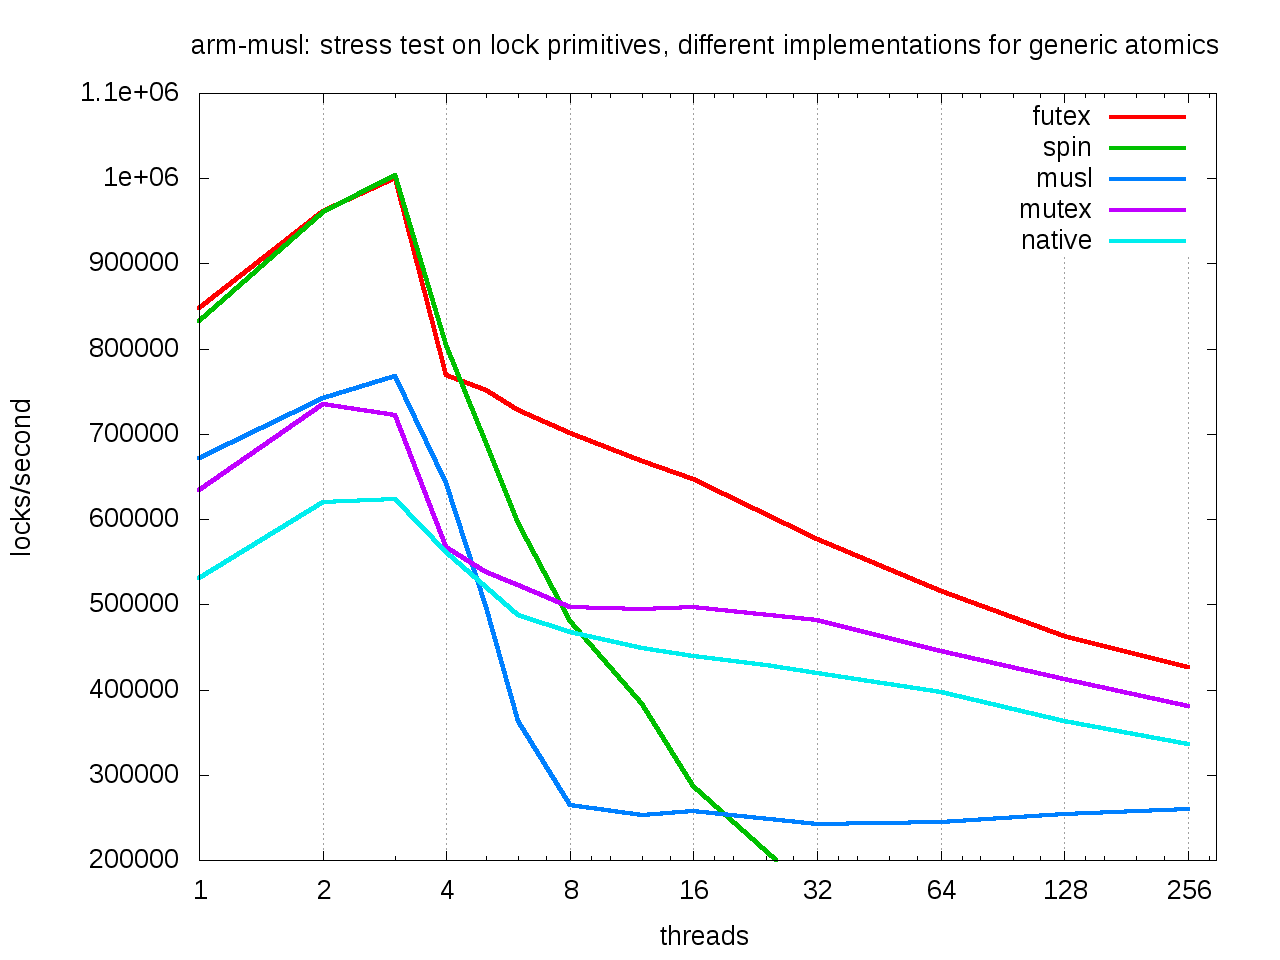
\includegraphics[width=0.48\textwidth]{benchs/arm/test-arm-u64.png}
  }%
  \subfigure[relative performance compared to mutex\label{fig:arm-rel}]{
    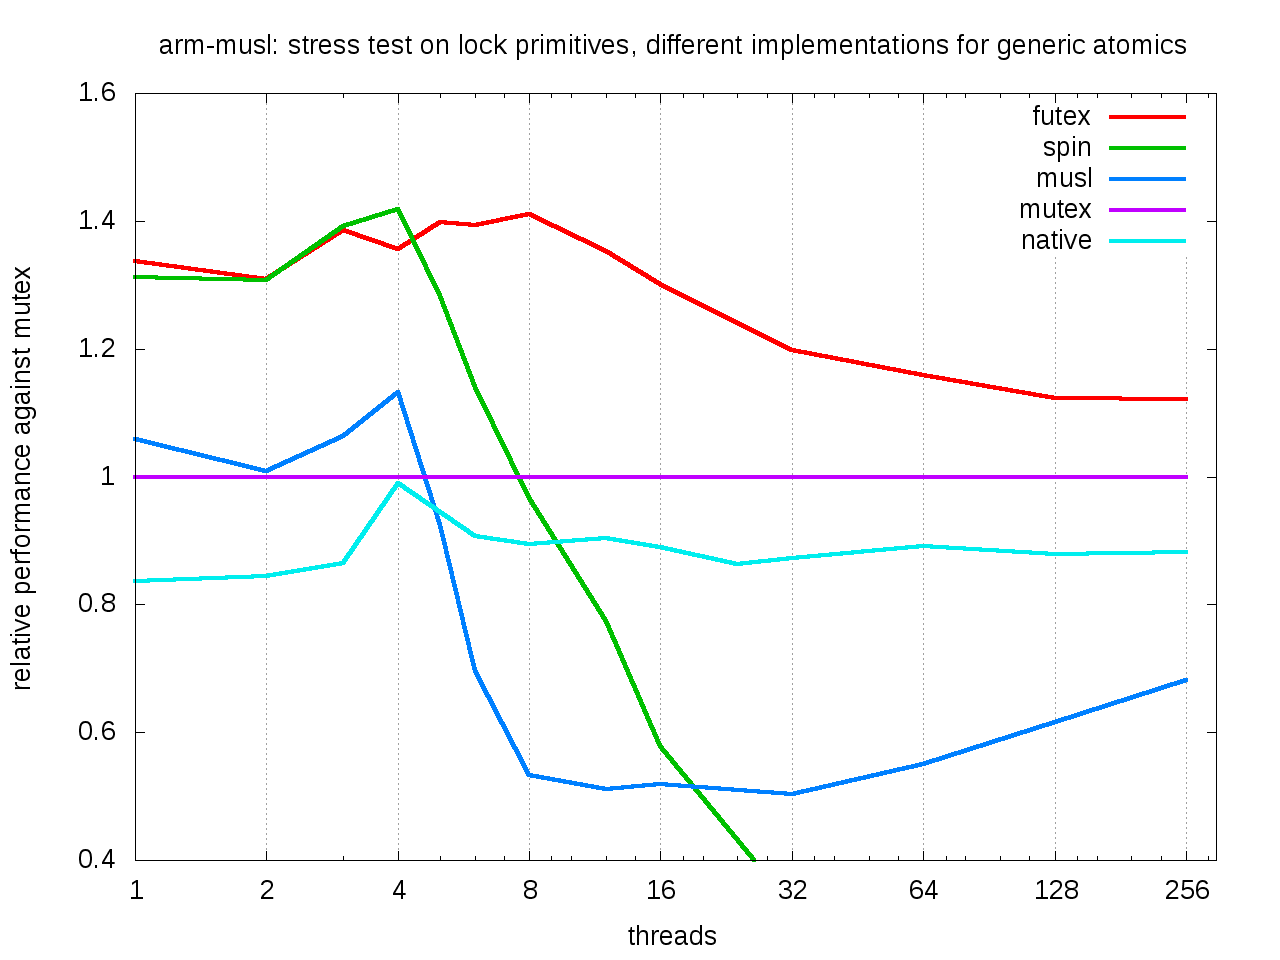
\includegraphics[width=0.48\textwidth]{benchs/arm/test-arm-u64-relative.png}
  }
  \caption{benchmarks on \texttt{arm}}
  \label{fig:arm}
\end{figure*}
\iflong%
\subsubsection{An \texttt{arm7} machine with 4 cores}
\label{sec-4-3-1}

This machine has 4 symmetric \texttt{arm7} cores at a \texttt{1.3 GHz} with \texttt{2
    GiB} of RAM. This system is equipped with Alpine Linux, so it has
\texttt{musl} as a native C library. The processor has atomic
instructions for word sizes up to 64 bit. The compiler is \texttt{gcc}
version \texttt{5.2}.
%
Here, the native C library is musl and so the atomic library of gcc are
compatible. Therefore the benchmarks include ``native''.


\subsubsection{A \texttt{x86\_64} machine with 2x2 hyperthreaded cores}
\label{sec-4-3-2}

This is a i7-4600U CPU at \texttt{2.10GHz} and with \texttt{8 GiB} of RAM. The
OS is Debian Linux, with \texttt{glibc} as native library.  The processor
has atomic instructions for word sizes up to 128 bit. The compiler
is \texttt{gcc} version \texttt{4.9}.
%
Because musl is not the native C library, the atomic library of gcc is not
compatible. Therefore the benchmark ``native'' is missing.

\subsection{Performance comparison}
\label{sec-4-4}
\else
\emph{Summarize platform and benchmark in one single paragraph.}
\emph{Summarize platform and benchmark in one single paragraph.}
\emph{Summarize platform and benchmark in one single paragraph.}
\emph{Summarize platform and benchmark in one single paragraph.}
\emph{Summarize platform and benchmark in one single paragraph.}
\emph{Summarize platform and benchmark in one single paragraph.}
\fi


The Fig.~\ref{fig:arm} shows the results on the \texttt{arm}
platform.
%
We see that all lock implementations allow for an acceleration of
the application when a small number of threads is used. But what is
also clear that the "native" lock performs worst for the case that
is the most interesting: the range where each thread has
its own CPU core at its disposal. Even the "mutex" lock performs better.

We also see that musl's internal lock structure shows a drastic
performance loss when it comes to congestion. This is due to a
switch of the spinning strategy: as soon as congestion is detected,
spinning is abandoned and threads directly attempt
\code{futex_wait}. This is meant to ensure fairness of lock acquisition,
but as we can see for our use case it has a dramatic impact on the
application throughput.

Here is the relative performance of the same experiments, where the
"mutex" implementation is taken as a base:

We see that our new implementation is about 60\% better than
the "native" version, or 40\% than a direct implementation with
mutex. It combines the good performance of a spinlock for the less
congested range with a good policy for strong congestion.

To finish let us consider the \texttt{x86\_64} platform. Although it
has more compute power than the other, the atomics of the hardware
are much less performing. This is due to the fact that here an
atomic instruction usually enforces a complete
synchronization at a cost of about 50 CPU cycles. Basically, the CPU
is blocked for this number of cycles. Compared to that, in a monitor based approach
as on the arm architecture part of these cycles can be used for other computations.
So on the \texttt{x86\_64} platform any atomic operation incurs a strong latency
penalty. Thereby, our application is not even able to accelerate for
2, 3 or 4 threads as it was the case on arm. In the contrary it
even decelerates.
Nevertheless the relative performance difference between the
different lock implementations look very similar.%
\footnote{Figures not shown, due to space limitations.}

\section{Conclusion}
\label{sec-5}

We have presented a new locking algorithm that combines consequent use
of C11 atomics with Linux' futex system calls. We have proven that it
is deadlock free, and that shows better
performance than other lock implementations.
\iflong
This is not surprising, an implementation that is tuned
for the purpose (very short CS) and that may avoid stacked calls into
the C library should always perform better than a generic one.
Surprising to us was the wide performance gap between the
implementations.
\fi

By pursuing this research we learned to mistrust some of the
urban legends that turn around atomics, futexes and lock structures in
general. At least when we stick to the basics (\code{futex_wait} and
\code{futex_wake}) and if we have a decent interface for atomics,
programming them is not as difficult as the legends suggest. Also
using a system call is not so much worse that spinning around an
atomic access. The performance factor between the two is only about
10, and so spinlocks in the order of 10 should be sufficient in many
cases.

This support library is now available as open source at
\url{http://stdatomic.gforge.inria.fr}. We hope to integrate it into the C library
that we used for most of our experiments, \texttt{musl}.

%%% -*-BibTeX-*-
%%% Do NOT edit. File created by BibTeX with style
%%% ACM-Reference-Format-Journals [18-Jan-2012].

%\bibliographystyle{ACM-Reference-Format-Journals}
%\bibliography{modernC}
\begin{thebibliography}{00}
\itemsep=0.8ex
%%% ====================================================================
%%% NOTE TO THE USER: you can override these defaults by providing
%%% customized versions of any of these macros before the \bibliography
%%% command.  Each of them MUST provide its own final punctuation,
%%% except for \shownote{}, \showDOI{}, and \showURL{}.  The latter two
%%% do not use final punctuation, in order to avoid confusing it with
%%% the Web address.
%%%
%%% To suppress output of a particular field, define its macro to expand
%%% to an empty string, or better, \unskip, like this:
%%%
%%% \newcommand{\showDOI}[1]{\unskip}   % LaTeX syntax
%%%
%%% \def \showDOI #1{\unskip}           % plain TeX syntax
%%%
%%% ====================================================================

\ifx \showCODEN    \undefined \def \showCODEN     #1{\unskip}     \fi
\ifx \showDOI      \undefined \def \showDOI       #1{{\tt DOI:}\penalty0{#1}\ }
  \fi
\ifx \showISBNx    \undefined \def \showISBNx     #1{\unskip}     \fi
\ifx \showISBNxiii \undefined \def \showISBNxiii  #1{\unskip}     \fi
\ifx \showISSN     \undefined \def \showISSN      #1{\unskip}     \fi
\ifx \showLCCN     \undefined \def \showLCCN      #1{\unskip}     \fi
\ifx \shownote     \undefined \def \shownote      #1{#1}          \fi
\ifx \showarticletitle \undefined \def \showarticletitle #1{#1}   \fi
\ifx \showURL      \undefined \def \showURL       #1{#1}          \fi

\bibitem[\protect\citeauthoryear{Alpine}{Alpine}{}]%
        {alpine}
{Alpine Linux}.
\newblock
\showURL{%
\url{http://alpinelinux.org/}}


\bibitem[\protect\citeauthoryear{Clang}{Clang}{2015}]%
        {clang}
{Clang}.
\newblock
\showURL{%
\url{http://clang.llvm.org/}}


\bibitem[\protect\citeauthoryear{gcc}{gcc}{2015}]%
        {gcc}
{gcc}.
\newblock {G}{N}{U} Compiler Collection.
\newblock
\showURL{%
\url{https://gcc.gnu.org/}}


\bibitem[\protect\citeauthoryear{glibc}{glibc}{2015}]%
        {glibc}
{glibc}.
\newblock {G}{N}{U} {C} library.
\newblock
\showURL{%
\url{https://www.gnu.org/software/libc/}}


\bibitem[\protect\citeauthoryear{Gustedt}{Gustedt}{2015}]%
        {gustedt15:futex}
{Jens Gustedt}. 2015.
\newblock {\em Futex based locks for C11's generic atomics}.
\newblock INRIA.
\newblock
\showURL{%
\url{https://hal.inria.fr/hal-0123xxxx}}


\bibitem[\protect\citeauthoryear{Hart}{Hart}{2009}]%
        {hart09}
{Darren Hart}. 2009.
\newblock \showarticletitle{A futex overview and update}.
\newblock {\em LWN.net\/} (2009).
\newblock
\showURL{%
\url{https://lwn.net/Articles/360699/}}


\bibitem[\protect\citeauthoryear{Hutton et~al\mbox{.}}{Hutton et~al\mbox{.}}{2002}]%
        {Hutton02fuss}
{Andrew~J. Hutton} et~al. 2002.
\newblock \showarticletitle{Fuss, Futexes and Furwocks: Fast Userlevel Locking
  in Linux}. In {\em Proceedings of the Ottawa Linux Symposium}. 479--495.
% \newblock
% \showURL{%
% \url{https://www.kernel.org/doc/ols/2002/ols2002-pages-479-495.pdf}}


\bibitem[\protect\citeauthoryear{IBM}{IBM}{1983}]%
        {IBM370}
IBM 1983.
\newblock {\em IBM System/370 Extended Architecture, Principles of Operation}.
\newblock IBM.
\newblock
\newblock
\shownote{SA22-7085.}


\bibitem[\protect\citeauthoryear{JTC1/SC22/WG14}{JTC1/SC22/WG14}{2011}]%
        {C11}
{JTC1/SC22/WG14} (Ed.). 2011.
\newblock {\em Programming languages~---~{C}\/} (cor. 1:2012 ed.).
\newblock Number ISO/IEC 9899. ISO.
% \newblock
% \showURL{%
% \url{http://www.open-std.org/jtc1/sc22/wg14/www/docs/n1570.pdf}}


\bibitem[\protect\citeauthoryear{Michael}{Michael}{2004}]%
        {michael04:aba}
{Maged~M. Michael}. 2004.
\newblock {\em {A}{B}{A} Prevention Using Single-Word Instructions}.
\newblock {T}ech. {R}ep. RC23089. IBM Research.
\newblock


\bibitem[\protect\citeauthoryear{MUSL}{MUSL}{}]%
        {musl}
{MUSL} libc.
\newblock
\showURL{%
\url{http://musl-libc.org}}


\bibitem[\protect\citeauthoryear{Netzer and Miller}{Netzer and Miller}{1992}]%
        {Netzer1992}
{Robert H.~B. Netzer} {and} {Barton~P. Miller}. 1992.
\newblock \showarticletitle{What Are Race Conditions? Some Issues and
  Formalizations}.
\newblock {\em ACM Lett. Program. Lang. Syst.\/} {1}, 1 (March 1992), 74--88.
\newblock
\showISSN{1057-4514}
% \showDOI{%
% \url{http://dx.doi.org/10.1145/130616.130623}}


\bibitem[\protect\citeauthoryear{POSIX}{POSIX}{2009}]%
        {POSIX2009}
{POSIX}. 2009.
\newblock {\em ISO/IEC/IEEE Information technology -- Portable Operating
  Systems Interface (POSIX®) Base Specifications}.
\newblock
\shownote{Issue 7.}
\newblock ISO, Geneva, Switzerland.


\end{thebibliography}
% Emacs 24.4.1 (Org mode 8.2.10)
\end{document}

%%% Local Variables:
%%% mode: latex
%%% mode: reftex
%%% fill-column: 75
%%% ispell-dictionary: "american"
%%% x-symbol-8bits: nil
%%% End:
